\documentclass[a4paper,10pt]{book}
\usepackage[english]{babel}     
\usepackage[utf8]{inputenc}     % accent symbols
\usepackage[T1]{fontenc}
\usepackage{lmodern}
\usepackage{microtype}
\usepackage{natbib}
\usepackage{tocbibind}          
\usepackage{amsmath}            % math symbols
\usepackage{amsthm}             % math symbols
\usepackage[colorlinks=true,linkcolor=red]{hyperref} % hyper link

% for code
\usepackage{listings}
\usepackage{color,xcolor}
\definecolor{mygreen}{rgb}{0,0.6,0}
\definecolor{mygray}{rgb}{0.9,0.9,0.9}
\definecolor{mymauve}{rgb}{0.58,0,0.82}
\lstset{
backgroundcolor=\color{mygray},
numbers=left,                    
columns=fullflexible,
breaklines=true,      
captionpos=b,         
tabsize=4,            
commentstyle=\color{mygreen}, 
escapeinside={\%*}{*)},       
keywordstyle=\color{blue},    
% stringstyle=\color{mymauve}\monaco,
frame=single,                        
rulesepcolor=\color{red!20!green!20!blue!20},
% identifierstyle=\color{red},
%% language=c++,
basicstyle=\tiny
}

\usepackage{indentfirst}
\setlength{\parindent}{2em}
\usepackage[onehalfspacing]{setspace}
% graph
\usepackage{pdfpages}
\usepackage{graphicx}
% box
\usepackage{booktabs}
\usepackage{tcolorbox}

%% user defined command
\newcommand{\keyword}[1]{\textbf{#1}}
\newcommand{\keywords}[1]{\textbf{#1}}
\newcommand{\lcmd}[1]{\texttt{#1}}
\newcommand{\head}[1]{\textnormal{\textbf{#1}}}
\newcommand{\itwords}[1]{\textit{#1}}

\usepackage{float}
% all symbols
\usepackage{tipa}
\usepackage{tipx}

\usepackage{datetime}
% \usepackage{movie15}


% variable
% TODO
\newcommand{\pdfauthor}{李明明}
\newcommand{\pdftitle}{工作}
\newcommand{\pdfsubject}{工作中的经验与教训}
\newcommand{\pdfkeywords}{工作经验与教训}
\newcommand{\bookname}{工作收获}
\newcommand{\bookoneword}{工作中吸取的经验和教训}
\newcommand{\timeandcompany}{2020年12月1日}

\usepackage{bm}
\usepackage{amsfonts}
\begin{document}


% Pages are numbered with lowercase Roman numbers.
% Chapters generate a table of contents entry but don't get a number.
\frontmatter{}
\newcommand{\mytitle}{Git}
\newcommand{\firstcreated}{Mar 16, 2023}

\begin{titlepage}

\newcommand{\HRule}{\rule{\linewidth}{0.5mm}} % Defines a new command for the horizontal lines, change thickness here

\center                         % Center everything on the page
 
%----------------------------------------------------------------------------------------
%	HEADING SECTIONS
%----------------------------------------------------------------------------------------


\includegraphics[width=0.5\textwidth]{logo}\\[1cm] % Include a department/university logo - this will require the graphicx package

%----------------------------------------------------------------------------------------
%	TITLE SECTION
%----------------------------------------------------------------------------------------

\HRule\\[0.4cm]
{ \huge \bfseries \mytitle}\\[0.4cm] % Title of your document
\HRule\\[1.5cm]
 
%----------------------------------------------------------------------------------------
%	AUTHOR SECTION
%----------------------------------------------------------------------------------------

\begin{minipage}{0.4\textwidth}
\begin{center} \large
Mingming \textsc{Li}\\ % Your name
\end{center}

\end{minipage}\\[2cm]


%----------------------------------------------------------------------------------------
%	DATE SECTION
% ----------------------------------------------------------------------------------------
\vfill
{\large First Created: \firstcreated}\\
{\large Last Modified: \today}\\[2cm] % Date, change the \today to a set date if you want to be precise



\end{titlepage}


%%% Local Variables:
%%% mode: latex
%%% Tex-master: "git"
%%% End:
\cleardoublepage{}
\phantomsection{}
\tableofcontents{}
\cleardoublepage{}
\phantomsection{}
\listoffigures{}
\cleardoublepage{}
\phantomsection{}
\listoftables{}


% Pages are numbered with Arabic numbers.
% Chapters are numbered and produce a table of contents entry.
\mainmatter{}

\part{Basics}
\label{part:basics}



\chapter{介绍}

在早期的人工智能中,我们处理和解决对人类来说难处理,但对机器来说很简单的,可以用正式的数学规则描述的问题。
而人工智能真正的挑战是那些对人类来说很简单,但难以正式的描述出的问题,比如识别说出的话或者图片中的人脸。

解决办法就是让机器从数据中进行学习,并以结构化的概念来理解这个世界,每个概念通过与更简单的概念的关系来定义。
如果我们画一个图来描述这些概念是如果在其他概念上构成的,该图就会很深,有很多层。
因此,也叫做深度学习。

最早的人工智能解决方式为:硬编码知识(hard-code knowledge)。
这种方式有一个知识库和一个推理机,
推理机由一系列逻辑推理规则组成,(人为设定)
通过将推理机应用与知识库来对世界进行理解,
这种方式未取得很大的成成功。



hard-code knowledge面临的难题是,AI系统需要有能力来获取知识,通过从原始数据中提取模式(pattern)。
这种能力就是机器学习。
一个简单的机器学习的算法为逻辑回归。


这些简单的机器学习算法的效率很大程度上依赖于数据的表征(representation),
表征中的每一个信息都称为特征(feature),
比如 [身高,体重,年龄,血压,心率...],
表征的选择对机器学习的效率有巨大的影响。

然而对于许多任务来说,我们很难知道需要提取什么特征。
比如,我们想识别图片中的汽车,我们可以使用汽车有轮子这个特征,但我们很难用像素来描述轮子,一个轮子有几何形状,但照片中的轮子受到光照,阴影,挡板和前景的障碍物的遮挡等等的影响。


一个解决方法为,使用机器学习来同时学习表征到输出的映射和表征本身,这个方法叫做“表征学习”。
学习得到的表征常常比手动设计的表征的准确率要高。
表征学习的经典算法为自编码器(autoencoder),
自编码器由编码函数(将输入数据转化为不同的表征)和解码函数(将新的表征转化为原始数据格式)组成。


当我们设计特征或者算法来学习特征的时候,我们的目标通常是将变量的因素(factors of variation)进行分离,而这因素可以解释观察到的数据。
在此处,因素指单独的影响源,该因素不是混合的,
它们可以被想象为我们用来理解数据中的复杂变化性的一种概念或者抽象,
例如,当我们分析一段录音,因素包括说话这的年龄,性别,口音和说话的内容等,
当我们分析汽车的照片,因素有汽车的位置,颜色,角度和太阳的亮度等。

一个主要的问题为,许多变量的因素同时影响着我们观测到的数据中的所有单个部分。
比如,红色轿车图片中的色素在晚上的时候非常接近黑色,阳光对整张图有着影响。

当然,我们很难从数据提取出高层次的抽象特征,比如口音,这需要对数据有专业的,人类水平的理解。
当获取表征的难度和解决问题的难度相似的时候,表征学习似乎对我们是没有帮助的。


深度学习通过引入使用更简单的表征表示的表征来解决表征学习中的核心问题。
深度学习是机器可以从更简单的概念中构建出更复杂的概念。
经典的深度学习算法为,“前馈深度网络”(feedforward deep network)或者多层感知机(multilayer perception)。


从基于规则的系统 $\rightarrow$ 机器学习 $\rightarrow{}$ 表征学习 $\rightarrow{}$ 深度学习的进化如图\ref{fig:introduction-deep-learning}所示:
\begin{figure}[!ht]
  \centering
  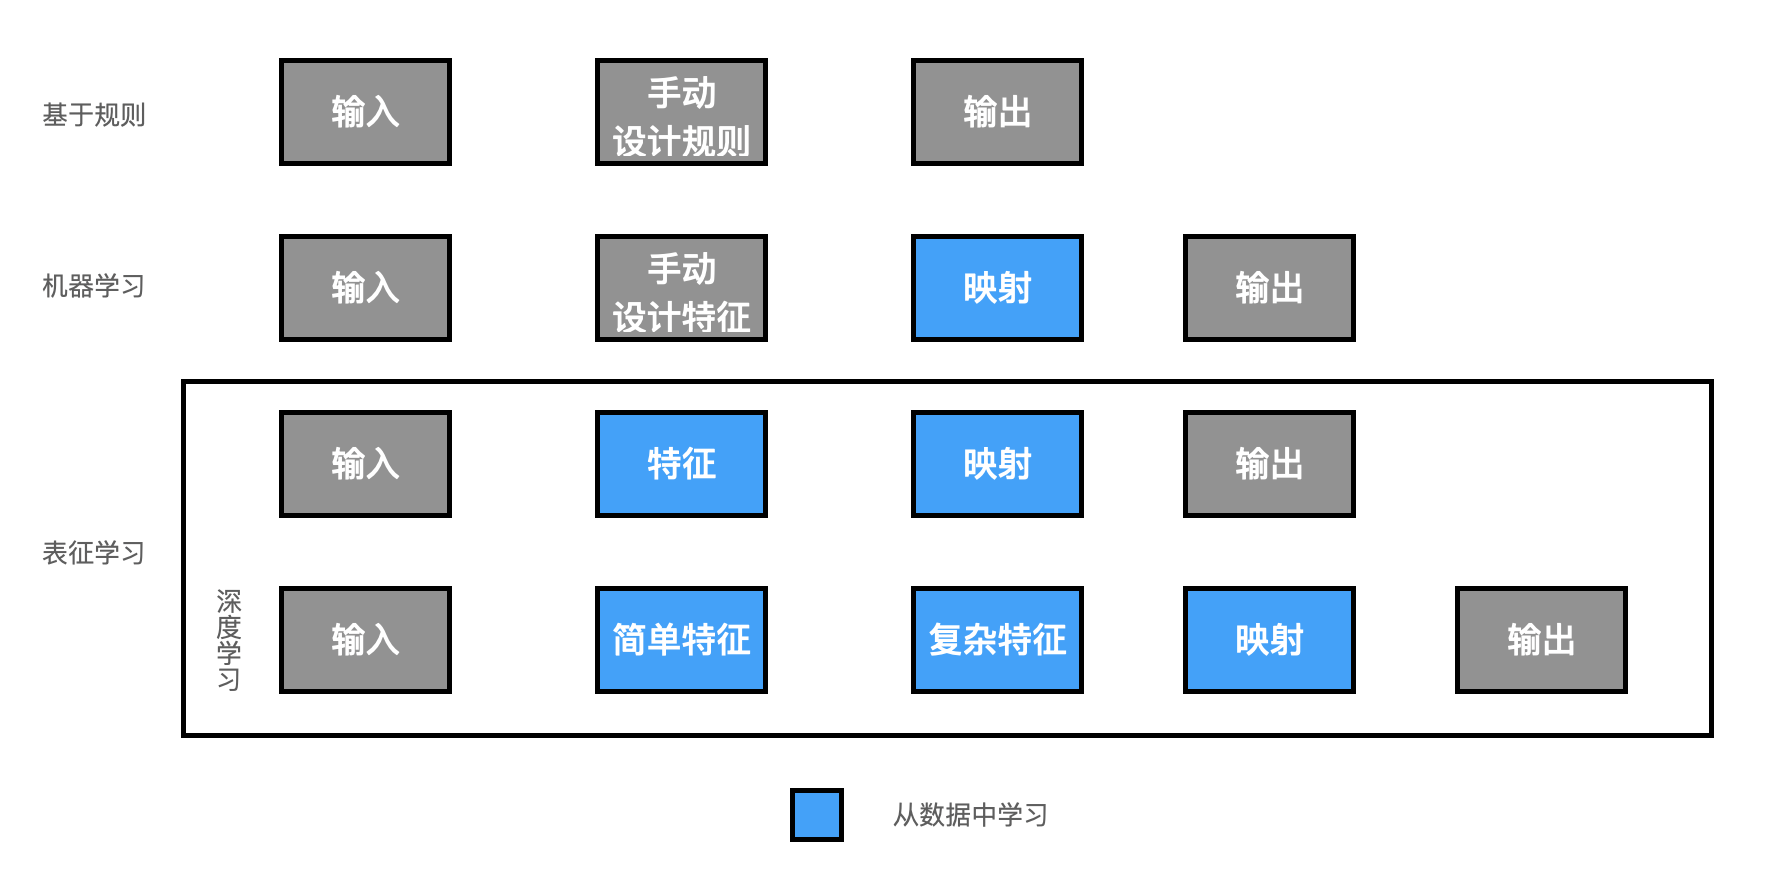
\includegraphics[width=\textwidth]{introduction-deep-learning.png}
  \caption{深度学习的进化}
  \label{fig:introduction-deep-learning}
\end{figure}








\chapter{Machine Learning Basics}


\section{Learning Algorithms}

A machine learning algorithm is an algorithm that is able to learn from data.
But what do we mean by learning?
Mitchell provides a succinct definition:
``A computer program is said to learn from experience $E$ with respect to some class of tasks $T$ and performance measure $P$, if its performance at tasks in $T$, as measured by $P$, improves with experience $E$''
Now, how does the learn happen?
The model or algorithm learns by adjusting the parameters contained in it.


\section{Capacity, Overfitting, Underfitting and Regularization}
We train model on training data but use test data (not used to train the model) to test out model.
The ability to perform on test data is called \keyword{generalization}.
We can use model on test data because we assume that the train data and the test has the same probability distribution (i.e. they have relationship).

The error on training data is called \keyword{training error}.
The error on test data is called \keyword{test error}.
Underfitting occurs when the model is not able to obtain a sufficient low error value on the training set.
Overfitting occurs when the gap between the training error and test error is too large.


We can control whether a model is more likely to overfit or underfit by altering its \keyword{capacity}.
The capacity is the pattern space (family of functions) we can learn from.

\keyword{Regularization} is any modification we make to a learnining algorithm that is intended to reduce its generalization error.

\begin{tcolorbox}
  Machine learning algorithm will generally perform best when their capacity is appropriate for the true complexity of the task and the amount of training data.
\end{tcolorbox}



\subsection{The No Free Lunch Theorem}


For any algorithms \(a_{1}\) and \(a_{2}\), at iteration step \(m\)
\begin{equation}
  \label{eq:1}
  \sum P(d_{m}^{y}|f,m,a_{1}) = \sum P(d_{m}^{y}|f,m,a_{2})
\end{equation}
where \(d_{m}^{y}\) denotes the ordered set of size \(m\) of the cost values \(y\) associated to input values \(x \in X\), \(f:X\longrightarrow Y\) is the function being optimized and \(P(d_{m}^{y}|f,m,a)\) is the conditional probability of obtaining a given sequence of cost values from algorithm \(a\) run \(m\) times on function \(f\).

The no free lunch theorem implies that we must design our machine learning algorithms to perform well on a specific task but not a universal task.


\section{Hyperparameters and validation sets}

\keyword{hyperparameters} are parameters used to control the algorithm's behavior but can or should not be learned by the learning algorithm.


In practice, we usually split training data into two disjoint subsets: training set and validation set (generally, 8:2n).
The validation set is used to adjust the hyperparameters.




\section{Building a machine learning algorithm}

Nearly all deep learning algorithms can be described as particular instances of a fairly simple recipe:
\begin{itemize}
\item a specification of a dataset
\item a cost function
\item an optimization procedure
\item a model
\end{itemize}





%%% Local Variables:
%%% mode: latex
%%% TeX-master: "deep-learning"
%%% End:


\chapter{Full Connected Networks}
\label{cha:full-conn-netw}

A fully connected neural network consists of a series of fully connected layers that connect every neuron in one layer to every neuron in the other layer.
Full connected neural network layers use matrix multiplication by a matrix of parameters with a separate parameter describing the interaction between each input unit and each output unit.
This means that every output unit interacts with every input unit.


Figure \ref{fig:fc} show the full connects neural network.
\begin{figure}[!htbp]
  \centering
  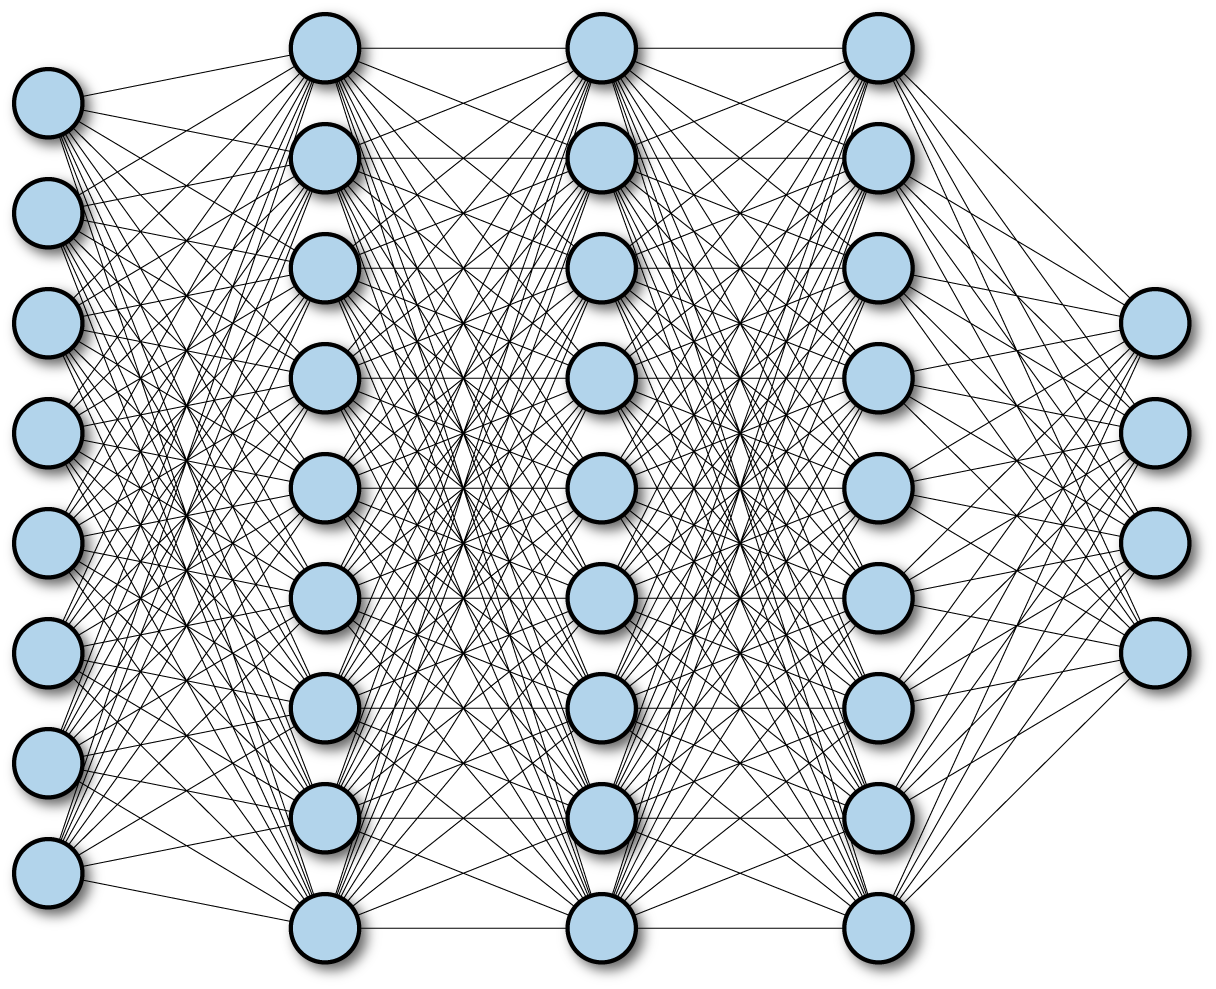
\includegraphics[width=0.8\textwidth]{fc}
  \caption{Full connected neural network}
  \label{fig:fc}
\end{figure}



%%% Local Variables:
%%% mode: latex
%%% TeX-master: "deep-learning"
%%% End:



\part{Computer Vision}
\label{part:build-mach-learn}


\chapter{CNN}

CNN stands for convolutional neural network.
Convolutional networks are neural networks that have convolutional layers.
A typical convolutional layer consists of three stages:
\begin{enumerate}
\item convolution stage: affine transform
\item detector stage: nonlinearty
\item pooling stage
\end{enumerate}

\section{Convolution}

\begin{equation}
  \label{eq:convolution}
  s(t) = \int x(a)w(t-a)da.
\end{equation}

This operation is called \keyword{convolution}.
The convolution operation is typically denoted with an asterisk:
\begin{equation}
  s(t) = (x*w)(t).
\end{equation}

In convolutional network terminology, the first argument (in this example, the function $x$) to the convolution is often referred to as the \keyword{input}, and the second argument (int this example, the function $w$) as the \keyword{kernel}.
The output is sometimes referred to as the \keyword{feature map}.

If we assume that $x$ and $w$ are defined only on integer $t$, we can define the discrete convolution:
\begin{equation}
  \label{eq:discrete-convolution}
  s(t) = (x*w)(t) = \sum_{a=-\infty}^{\infty} x(a)w(t-a).
\end{equation}

We often use convolutions over more than one axis at a time.
For example, if we use a two-dimensinal image $I$ as our input, we probably also want to use a two-dimensional kernel $K$:
\begin{equation}
  S(i,j) = (I*K)(i,j) = \sum_m\sum_n I(m,n)K(i-m,j-n).
\end{equation}


The following formula can be used to calculate the output dimension.
\begin{gather}
  h_{o} = \frac{h_{i} - h_{k}}{h_{s}} + 1\\
  w_{o} = \frac{w_{i} - w_{k}}{w_{s}} + 1
\end{gather}
where \(h_{o}\) is the output height, \(h_{i}\) is the input height, \(h_{k}\) is the kernel height, \(h_{s}\) is the stride height, \(w_{o}\) is the output width, \(w_{i}\) is the input width, \(w_{k}\) is the kernel width, \(w_{s}\) is the stride width.

The convolution operation is shown in Figure \ref{fig:conv-op}.
\begin{figure}[!htbp]
  \centering
  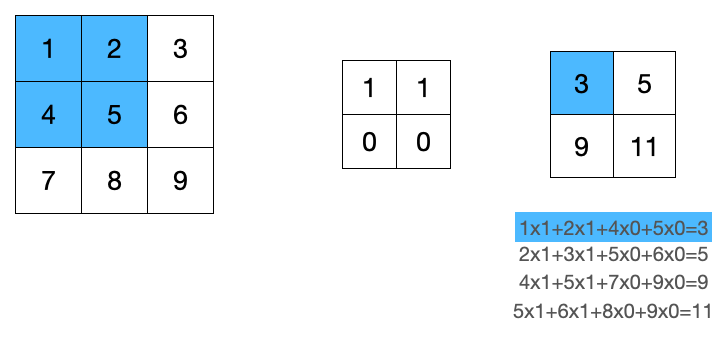
\includegraphics[width=0.8\textwidth]{conv}
  \caption{Convoluation operation}
  \label{fig:conv-op}
\end{figure}
\section{Properties}

CNN leverages three important ideas:
\begin{itemize}
\item sparse interaction.
\item parameter sharing.
\item equivariant representations.
\end{itemize}

\subsection{Sparse interaction}

This is accomplished by making the kernel smaller than the input.


\subsection{Parameter sharing}

In convolutional layers, the same parameter defined in one kernel are used at every position of the input.


\subsection{Equivariant representations}

In the case of convolution, the particular form of a parameter sharing causes the layer to have a property called \keyword{equivariance} to translation.
To say a function is equivariant means that if the input changes, the output changes in the same way.




\section{ Pooling}


A pooling function replaces the output of the net at a certain location with a summary statistic of the nearby outputs.
For example, the max pooling oeration reports the maximum output within a rectangular neighborhood.
Pooling helps to make the representation approximately invariant to small translations of the input.
Invariant to translation means that if we translate the input by a small amount, the values of most of the pooled outputs do not change.

The following formula can be used to calculate the output dimension.
\begin{gather}
  h_{o} = \frac{h_{i} - h_{k}}{h_{s}} + 1\\
  w_{o} = \frac{w_{i} - w_{k}}{w_{s}} + 1
\end{gather}
where \(h_{o}\) is the output height, \(h_{i}\) is the input height, \(h_{k}\) is the pooling height, \(h_{s}\) is the stride height, \(w_{o}\) is the output width, \(w_{i}\) is the input width, \(w_{k}\) is the pooling width, \(w_{s}\) is the stride width.


%%% Local Variables:
%%% mode: latex
%%% TeX-master: "machine-learning"
%%% End:


\part{Natural Language Processing}
\label{part:natur-lang-proc-1}


\chapter{Text Preprocessing}
\label{cha:text-preprocessing}

To convert text to a data format that is easier for computer to train a model, we need text preprocessing.
Here are the common preprocessing steps for text:
\begin{enumerate}
\item Load text as strings into memory.
\item Split strings into tokens (e.g., words or characters).
\item Build a table of vocabulary to map the split tokens to numerical indices.
\item Convert text into sequences of numerical indices.
\end{enumerate}


A \keyword{token} is the basic unit in text, for example, word or character.
The string type of the token is inconvenient to be used by models.
We build a dictionary called vocabulary to map string tokens into numerical indices starting from 0.
To do so, we first count the unique tokens in all the documents from the training set, namely a \keyword{corpus}, and then assign a numerical index to each unique token according to its frequency.
Rarely appeared tokens are often removed to reduce the complexity.
Any token that does not exist in the corpus or has been removed is mapped into a special unknown token "<unk>".
We can also add a list of reserved tokens, such as “<pad>” for padding, “<bos>” to present the beginning for a sequence, and “<eos>” for the end of a sequence.




%%% Local Variables:
%%% mode: latex
%%% TeX-master: "deep-learning"
%%% End:


\chapter{Language Model}
\label{cha:language-model}

The goal of a language model is to estimate the joint probability of the sequence
\begin{equation}
  \label{eq:language-model}
  P(x_{1},\ldots,x_{T})
\end{equation}
Where \(T\) is a constant.


Generally, the probability of \((x_{1},\ldots,x_{T})\) is:
\begin{equation}
  \label{eq:language-model-p}
  P(x_{1},\ldots,x_{T}) = \prod_{t=1}^{T}P(x_{t}|x_{t-1},\ldots,x_{1})
\end{equation}

\section{Markov Model}
\label{sec:markov-model}


In probability theory, a Markov model is a stochastic model used to model pseudo-randomly changing systems.
It is assumed that future states depend only on the current state, not on the events that occurred before it (that is, it assumes the Markov property).
Generally, this assumption enables reasoning and computation with the model that would otherwise be intractable.

Where \(T\) is a constant.



The simplest Markov model is the Markov chain.
\begin{equation}
  \label{eq:markov-chain}
  P(x_{t}|x_{1},\ldots,x_{t-1}) = P(x_{t}|x_{t-1})
\end{equation}

In this case, we have a \keyword{first-order Markov model} and \(P(x)\) is given by:
\begin{equation}
  \label{eq:first-order-markov-model}
  P(x_{1},\ldots,x_{T}) = \prod_{t=1}^{T} P(x_{t}|x_{t-1}).
\end{equation}

\section{n-grams}
\label{sec:n-grams}

\begin{gather}
  \label{eq:n-gram-1}
  P(x_{1},\ldots,x_{T}) = \prod_{t-1}^{T} P(x_{t})\\
  \label{eq:n-gram-2}
  P(x_{1},\ldots,x_{T}) = \prod_{t-1}^{T} P(x_{t}|x_{t-1})\\ 
  \label{eq:n-gram-3} 
  P(x_{1},\ldots,x_{T}) = \prod_{t-1}^{T} P(x_{t}|x_{t-1},x_{t-2})
\end{gather}

Formula \ref{eq:n-gram-1} \ref{eq:n-gram-2} and \ref{eq:n-gram-3} refers to \keyword{unigram}, \keyword{bigram} and \keyword{trigram}.




%%% Local Variables:
%%% mode: latex
%%% TeX-master: "deep-learning"
%%% End:


\chapter{RNN}
\label{cha:rnn}

RNN stands for recurrent neural network.
RNN is neural network that has recurrent layers.
While CNNs can efficiently process spatial information, RNNs are designed to better handle sequential information.
RNNs introduce state variables to store past information, together with the current inputs, to determine the current outputs.

\section{Recurrent}
\label{sec:recurrent}

\begin{equation}
  \label{eq:3}
  s^{(t)} = f(s^{(t-1)}; \theta)
\end{equation}
Where \(s^{(t)}\) is the state or output at time \(t\), \(f\) is the function, \(\theta\) is the parameter.
Equation \ref{eq:3} is recurrent because \(s\) at time \(t\) refer to itself at time \(t-1\).


\begin{equation}
  \label{eq:4}
  s^{(t)} = f(s^{(t-1)}, x^{(t)}; \theta)
\end{equation}
This equation is similar to equation \ref{eq:3} but with input \(x^{(t)}\).


In natural language processing (NLP), we usually need to compute
\begin{equation}
  \label{eq:nlp}
  P(x_{t}|x_{t-1},\ldots,x_{1})
\end{equation}

With n-gram model (Section \ref{sec:n-grams}), the number of model parameters increase exponentially as n increase.
We need to store \(|V|^{n}\) numbers for a vocabulary set \(V\).
In this case, we usually use a latent variable model:
\begin{equation}
  \label{eq:rnn-model}
  P(x_{t}|x_{t-1},\ldots,x_{1}) \approx P(x_{t}|h_{t-1})
\end{equation}
and
\begin{equation}
  \label{eq:latent}
  h_{t} = f(x_{t},h_{t-1})
\end{equation}


\section{Properties}
\label{sec:properties}


RNN leverages three important ideas:
\begin{itemize}
\item sparse interaction.
\item parameter sharing.
\item 
\end{itemize}

\subsection{Sparse interaction}
\label{sec:sparse-interaction}


Comparing to traditional neural network, it has sparse interaction.
For example, in Equation \ref{eq:4}, \(s^{(t)}\) is determined by \(s^{(t-1)}\) and \(x^{(t)}\).
It has no direct interaction with \(x^{(1)}, x^{(2)}, \ldots x^{(t-1)}\) because they are contained in \(s^{(t-1)}\).


\subsection{Parameter sharing}
\label{sec:parameter-sharing}

In recurrent layers, the same parameters defined in function \(f\) are used at every position of the input.






%%% Local Variables:
%%% mode: latex
%%% TeX-master: "deep-learning"
%%% End:


\part{Computer Vision Practice}
\label{part:comp-visi-pract}

\chapter{Classification}

Image classification comprises two major part: CNN network part and full connected network part.


CNN network is used to extract feature maps from the images.
Feature maps contains the information used to classifier the image.
The FC network output n-class dimension vector, each dimension for a class probability.


\section{LeNet with Keras}

The LeNet architecture is a seminal work in the deep learning community, first introduced by LeCun et al. in their 1998 paper, Gradient-Based Learning Applied to Document Recognition \cite{YL98}.

\label{sec:lenet-with-keras}



The code is on \href{https://github.com/mingmingli916/cv_classification}{Github}.


\subsection{Error and Anylysis}

At first, the division value used is 255.0 (train.py line 35).
Normally, this should make sense, becuase the value of image points lay in [0,255].
The output is as shown in Figure \ref{fig:div255-epochs20} (epochs=20) and \ref{fig:div255-epochs100} (epochs=100).
\begin{figure}[!ht]
  \centering
  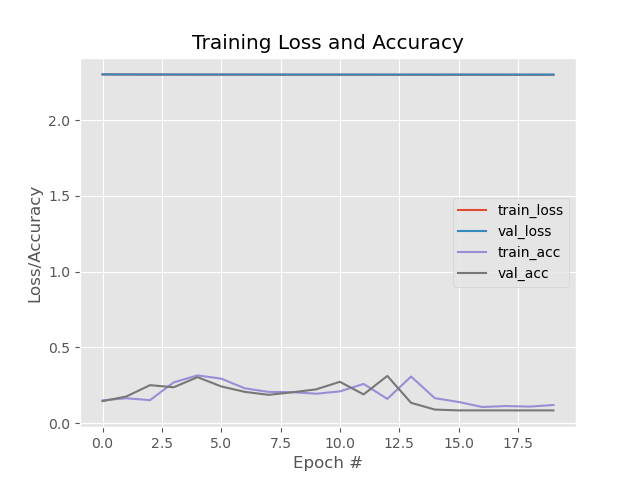
\includegraphics[width=0.8\textwidth]{epochs20_div255}
  \caption{Divide 255 and epochs=20}
  \label{fig:div255-epochs20}
\end{figure}


\begin{figure}[!ht]
  \centering
  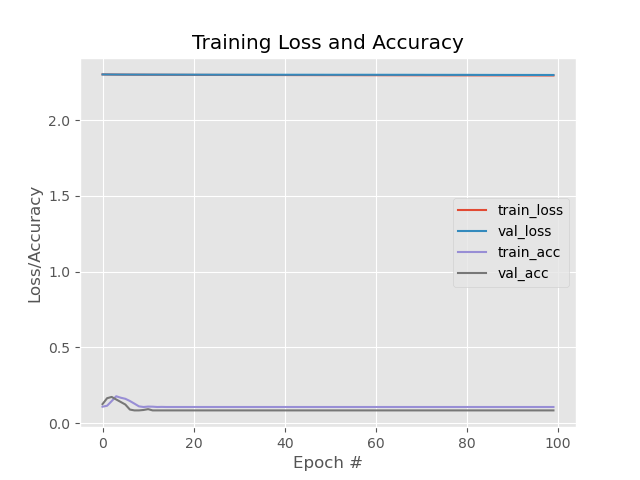
\includegraphics[width=0.8\textwidth]{epochs100_div255}
  \caption{Divide 255 and epochs=100}
  \label{fig:div255-epochs100}
\end{figure}


After diving into the dataset, I found that the maximum value is 16.
After changing the division to 16, the result is shown in Figure \ref{fig:div16-epochs20}.

\begin{figure}[!ht]
  \centering
  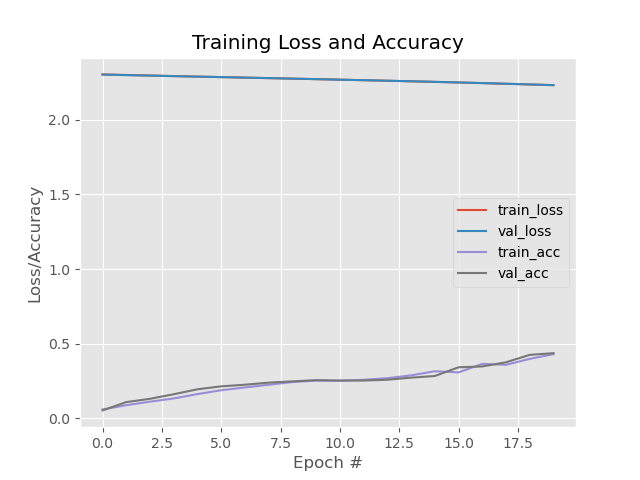
\includegraphics[width=0.8\textwidth]{epochs20_div16}
  \caption{Divide 16 and epochs=20}
  \label{fig:div16-epochs20}
\end{figure}


From the Figue \ref{fig:div16-epochs20} we can see that the epochs is too small.
After chaning the epochs to 100, the result is shown inf Figure \ref{fig:div16-epochs100}.
\begin{figure}[!ht]
  \centering
  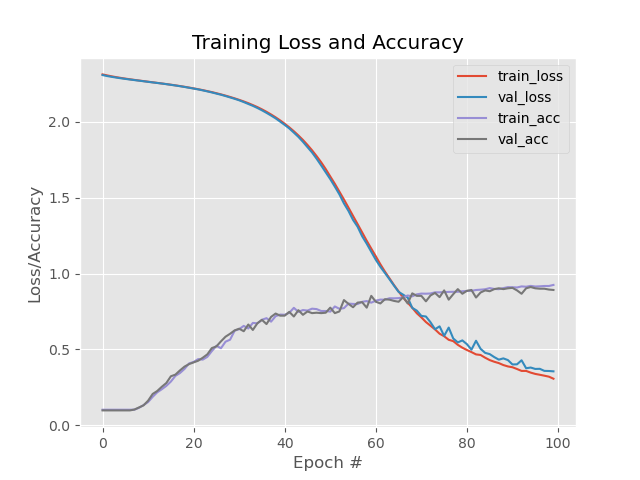
\includegraphics[width=0.8\textwidth]{epochs100_div16}
  \caption{Divide 16 and epochs=100}
  \label{fig:div16-epochs100}
\end{figure}


\section{LeNet with PyTorch}
\label{sec:lenet-with-pytorch}

The code link on \href{https://github.com/mingmingli916/dl_classification}{Github}.

Before, there is no tensorboard in PyTorch. You did the training process visualization.
With the tensorboard, it becomes more easier for the visualization in training process.



%%% Local Variables:
%%% mode: latex
%%% TeX-master: "deep-learning"
%%% End:


\chapter{Object Detection}

Usually, there are often multiple objects in the image of interest.
We not only want to know their categories, but also their specific positions in the image.
In computer vision, we refer to such tasks as object detection (or object recognition).


\section{Single-Shot Detector}
\label{sec:single-shot-detector}



The object dection model used here is the SSD\footnote{\url{https://arxiv.org/pdf/1512.02325.pdf}}.

The code is on \href{https://github.com/mingmingli916/object_detection_pytorch}{Github}.


Figure \ref{fig:sd} show the structure.
\begin{figure}[!htbp]
  \centering
  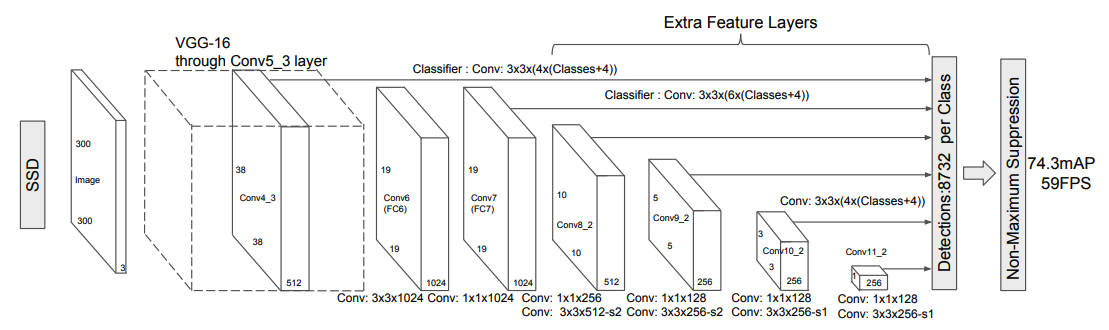
\includegraphics[width=0.9\textwidth]{ssd}
  \caption{SSD}
  \label{fig:ssd}
\end{figure}

There are two parts: backbone and SSD head.
The backbone is the EGG as the feature extractor.
The SSD head is a set of convolution layers.
The SSD head extracts features on different size.
Then it do regression and classification to achieve anchor box offset and object class.

\subsection{Bounding box}
\label{sec:bounding-box}


In object detection, we usually use a \keyword{bounding box} to describe the spatial location of an object.
The bounding box is rectangular, which is determined by the $x$ and $y$ coordinates of the upper-left corner of the rectangle and the such coordinates of the lower-right corner.
Another commonly used bounding box representation is the $(x, y)$-axis coordinates of the bounding box center, and the width and height of the box.

For example in Figure \ref{fig:bounding-box}.
\begin{figure}[!ht]
  \centering
  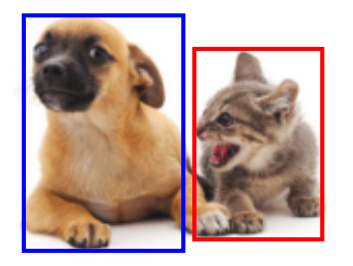
\includegraphics[width=0.7\textwidth]{bounding-box.png}
  \caption{Bounding box}
  \label{fig:bounding-box}
\end{figure}



\subsection{Anchor boxes}
\label{sec:anchor-boxes}

Object detection algorithms usually sample a large number of regions in the input image, determine whether these regions contain objects of interest, and adjust the boundaries of the regions so as to predict the ground-truth bounding boxes of the objects more accurately.

Different models may adopt different region sampling schemes.
One method is: it generates multiple bounding boxes with varying scales and aspect ratios centered on each pixel.
These bounding boxes are called \keyword{anchor boxes}. 



Suppose that the input image has a height of $h$ and width of $w$.
We generate anchor boxes with different shapes centered on each pixel of the image.
Let the scale be $s \in (0, 1]$ and the aspect ratio (ratio of width to height) is $r > 0$.
Left out the scale $s$ and the anchor box area does not change.
The new width and height of the anchor box are $w\sqrt{r}$ and $h/\sqrt{r}$ respectively.
Counting the scale $s$, those are $ws\sqrt{r}$ and $h/\sqrt{r}$ respectively.
Note that when the center position is given, an anchor box with known width and height is determined.


To generate multiple anchor boxes with different shapes, let us set a series of scales $s_{1}, \dots, s_{n}$ and a series of aspect ratios $r_{1}, \dots,r_{m}$.
When using all the combinations of these scales and aspect ratios with each pixel as the center, the input image will have a total of $whnm$ anchor boxes.
Although these anchor boxes may cover all the ground-truth bounding boxes, the computational complexity is easily too high.
In practice, we can only consider those combinations containing $s_{1}$ and $r{1}$:
\begin{equation}
  \label{eq:1}
  (s_{1}, r_{1}), (s_{1}, r_{2}), \dots, (s_{1}, r_{m}), (s_{2}, r_{1}), (s_{3}, r_{1}), \dots, (s_{n}, r_{1})
\end{equation}
That is to say, the number of anchor boxes centered on the same pixel is $n + m - 1$.
For the entire input image, we will generate a total of $wh(n + m - 1)$ anchor boxes.

For example in Figure
\begin{figure}[!ht]
  \centering
  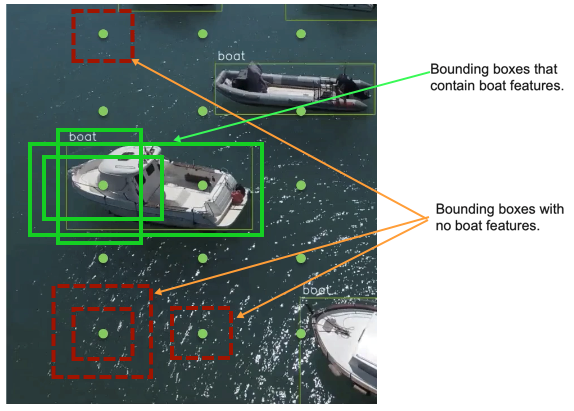
\includegraphics[width=0.8\textwidth]{anchor-boxes.png}
  \caption{Anchor boxes}
  \label{fig:anchor-boxes}
\end{figure}


\subsection{IntersectionoverUnion(IoU)}
\label{sec:iou}

We use IoU to measure the similarity between the anchor boxes and the ground-truth bounding box.


\subsection{Labeling Anchor Boxes in Training Data}
\label{sec:label-anch-boxes}

In a training dataset, we consider each anchor box as a training example.
In order to train an object detection model, we need class and offset labels for each anchor box.


To label any generated anchor box, we refer to the labeled location and class of its assigned ground-truth bounding box that is closest to the anchor box.

Given an image,suppose that the anchor boxes are \(A_{1}, A_{2}, \ldots A_{n_{a}}\) and the ground-truth bounding boxes are \(B_{1},B_{2},\ldots B_{n_{b}}\), where \(n_{a} \ge n_{b}\).
Let us define a matrix \(X \in R_{n_{a}\times n_{b}}\), whose element \(x_{ij}\) in the \(i^{th}\) row and \(j^{th}\) column is the IoU of the anchor box \(A_{i}\) and the ground-truth bounding box \(B_{j}\).
The algorithm consists of the following steps:

\begin{enumerate}
\item \label{item:1}Find the largest element in matrix \(X\) and denote its row and column indices as \(i_{1}\) and \(j_{1}\), respectively. Then the ground-truth bounding box \(B_{j_{1}}\) is assigned to the anchor box \(A_{i_{1}}\). After the first assignment, discard all the elements in the \(i_{1}^{th}\) row and the \(j_{1}^{th}\) column in matrix \(X\).
\item Repeat process \ref{item:1} until all elements in \(n_{b}\) columns in matrix \(X\) are discarded. 
\item Traverse through the remaining \(n_{a} - n_{b}\) anchor boxes. For example, given any anchor box \(A_{i}\), find the ground-truth bounding box \(B_{j}\) with the largest IoU with \(A_{i}\) throughout the \(i^{th}\) row of matrix \(X\), and assign \(B_{j}\) to \(A_{i}\) only if this IoU is greater than a predefined threshold.
\end{enumerate}

\subsection{Labeling Classes and Offsets}
\label{sec:label-class-offs}

Suppose that an anchor box A is assigned a ground-truth bounding box B.
On one hand, the class of the anchor box A will be labeled as that of B.
On the other hand, the offset of the anchor box A will be labeled according to the relative position between the central coordinates of B and A together with the relative size between these two boxes.
Here's a command transformation.
Given the central coordinates of A and B as \((x_{a}, y_{a})\) and \((x_{b},y_{b})\), their widths as \(w_{a}\) and \(w_{b}\), and their heights as \(h_{a}\)a nd \(h_{b}\), respectively.
We label the offset of A as:
\begin{equation}
  \label{eq:2}
  \bigl(
  \frac{\frac{x_{b}-x_{a}}{w_{a}}-\mu_{x}}{\sigma_{x}},   \frac{\frac{y_{b}-y_{a}}{h_{a}}-\mu_{y}}{\sigma_{y}},
  \frac{\log\frac{w_{b}}{w_{a}}-\mu_{w}}{\sigma_{w}},  \frac{\log\frac{h_{b}}{h_{a}}-\mu_{h}}{\sigma_{h}}
  \bigr)
\end{equation}
where default values of the constants are \(\mu_{x}=\mu_{y}=\mu_{w}=\mu_{h}=0, \sigma_{x}=\sigma_{y}=0.1\) and \(\mu_{w}=\mu_{h}=0.2\).




\section{R-CNN models}

\subsection{Region-based CNN (R-CNN)}
\label{sec:region-based-cnn}

The R-CNN consists of the following four steps:
\begin{enumerate}
\item Perform \keyword{selective search} to extract multiple high-quality \keyword{region proposals} on the input image.
  These proposed regions are usually selected at multiple scales with different shapes and sizes.
  Each region proposal will be labeled with a class and a ground-truth bounding box.
\item Choose a pretrained CNN and truncate it before the output layer.
  Resize each region proposal to the input size required by the network, and output the extracted features for the region proposal through forward propagation.
\item Take the extracted features and labeled class of each region proposal as an example.
  Train multiple \keyword{support vector machines} to classify objects, where each support vector machine individually determines whether the example contains a specific class.
\item Take the extracted features and labeled bounding box of each region proposal as an example.
  Train a \keyword{linear regression} model to predict the ground-truth bounding box.
\end{enumerate}

\begin{figure}[H]
  \centering
  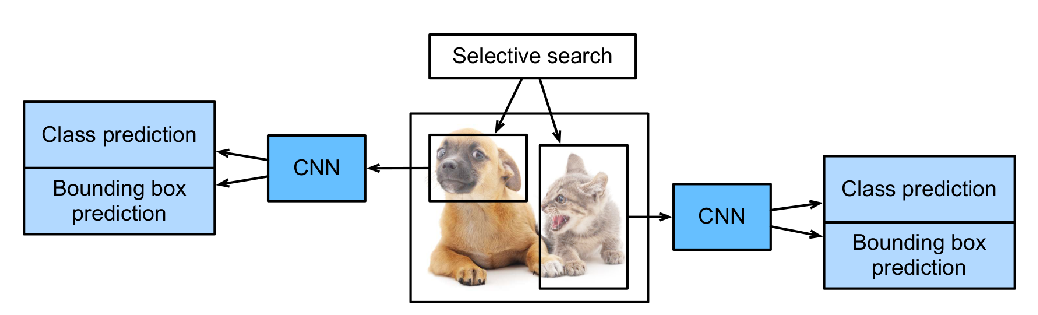
\includegraphics[width=0.8\textwidth]{rcnn}
  \caption{R-CNN}
  \label{fig:r-cnn}
\end{figure}

Although the R-CNN model uses pretrained CNNs to effectively extract image features, it is slow.
Imagine that we select thousands of region proposals from a single input image: this requires thousands of CNN forward propagations to perform object detection.
This massive computing load makes it infeasible to widely use R-CNNs in real-world applications.


\subsection{Fast R-CNN}
\label{sec:fast-r-cnn}

The main performance bottleneck of an R-CNN lies in the independent CNN forward propagation for each region proposal, without sharing computation.
Since these regions usually have overlaps, independent feature extractions lead to much repeated computation.
One of the major improvements of the fast R-CNN from the R-CNN is that the CNN forward prop- agation is only performed on the entire image.

\begin{figure}[H]
  \centering
  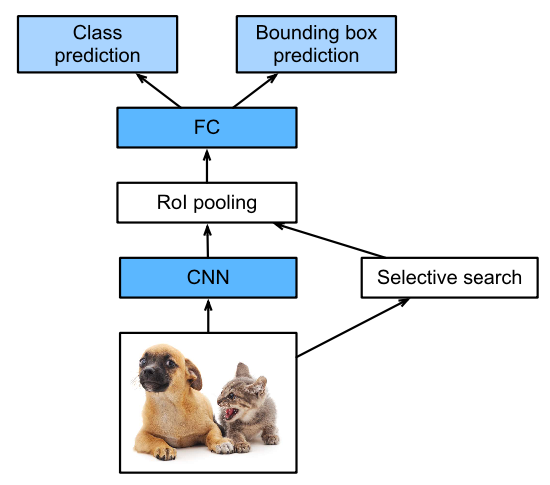
\includegraphics[width=0.8\textwidth]{fast-rcnn}
  \caption{Fast R-CNN}
  \label{fig:fast-rcnn}
\end{figure}

Its major computations are as follows:
\begin{enumerate}
\item Compared with the R-CNN, in the fast R-CNN the input of the CNN for feature extraction is the entire image, rather than individual region proposals.
  Moreover, this CNN is trainable.
  Given an input image, let the shape of the CNN output be \(1 \times c \times h_{1} \times w_{1}\).
\item Suppose that selective search generates n region proposals.
  These region proposals (of different shapes) mark \keyword{regions of interest} (of different shapes) on the CNN output.
  Then these regions of interest further extract features of the same shape (say height \(h_{2}\) and width \(w_{2}\) are specified) in order to be easily concatenated.
  To achieve this, the fast R-CNN introduces the \keyword{region of interest (RoI)} pooling layer: the CNN output and region proposals are input into this layer, outputting concatenated features of shape \(n \times c \times h_{2} \times w_{2}\) that are further extracted for all the region proposals.
\item Using a fully connected layer,transform the concatenated features into an output of shape \(n \times d\), where \(d\) depends on the model design.
\item Predict the class and bounding box for each of the n region proposals.
  More concretely, in class and bounding box prediction, transform the fully connected layer output into an output of shape \(n \times q\) (q is the number of classes) and an output of shape \(n \times 4\), respectively.
\end{enumerate}

\subsection{Faster R-CNN}
\label{sec:faster-r-cnn}

To be more accurate in object detection, the fast R-CNN model usually has to generate a lot of region proposals in selective search.
To reduce region proposals without loss of accuracy, the faster R-CNN proposes to replace selective search with a \keyword{region proposal network}.

\begin{figure}[H]
  \centering
  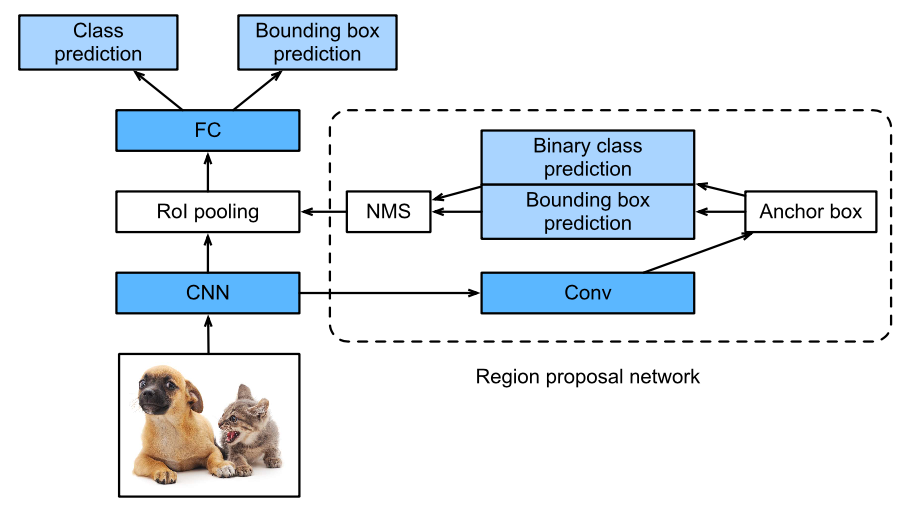
\includegraphics[width=0.8\textwidth]{faster-rcnn}
  \caption{Faster R-CNN}
  \label{fig:faster-rcnn}
\end{figure}

The region proposal network works in the following steps:
\begin{enumerate}
\item Use a \(3 × 3\) convolutional layer with padding of 1 to transform the CNN output to a new output with c channels.
  In this way, each unit along the spatial dimensions of the CNN-extracted feature maps gets a new feature vector of length c.
\item Centered on each pixel of the feature maps, generate multiple anchor boxes of different scales and aspect ratios and label them.
\item Using the length-c feature vector at the center of each anchor box,predict the binary class (background or objects) and bounding box for this anchor box.
\item Consider those predicted bounding boxes whose predicted classes are objects.
  Remove overlapped results using non-maximum suppression.
  The remaining predicted bounding boxes for objects are the region proposals required by the region of interest pooling layer.
\end{enumerate}


\subsection{Mask R-CNN}
\label{sec:mask-r-cnn}

In the training dataset, if pixel-level positions of object are also labeled on images, the mask R-CNN can effectively leverage such detailed labels to further improve the accuracy of object detection.


\begin{figure}[H]
  \centering
  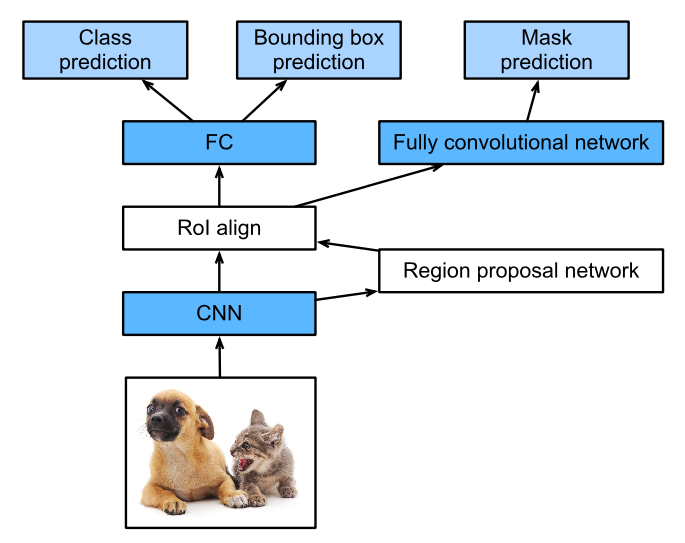
\includegraphics[width=0.8\textwidth]{mask-rcnn}
  \caption{Mask R-CNN}
  \label{fig:mask-rcnn}
\end{figure}

The mask R-CNN replaces the region of interest pooling layer with the \keyword{region of interest (RoI) alignment} layer.
This region of interest alignment layer uses bilinear interpolation to preserve the spatial information on the feature maps, which is more suitable for pixel-level prediction.
The output of this layer contains feature maps of the same shape for all the regions of interest.
They are used to predict not only the class and bounding box for each region of interest, but also the pixel-level position of the object through an additional fully convolutional network.

%%% Local Variables:
%%% mode: latex
%%% TeX-master: "deep-learning"
%%% End:


\chapter{Segmentation}

\section{Image Segmentation and Instance Segmentation}
\label{sec:image-segm-inst}

Image segmentation divides an image into several constituent regions.
The methods for this type of problem usually make use of the correlation between pixels in the image.
It does not need label information about image pixels during training, and it cannot guarantee that the segmented regions will have the semantics that we hope to obtain during prediction.

Instance segmentation is also called simultaneous detection and segmentation.
It studies how to recognize the pixel-level regions of each object instance in an image.
Different from semantic segmentation, instance segmentation needs to distinguish not only semantics, but also different object instances.


\section{Full Convolutional Network}
\label{sec:full-conv-netw}


Semantic segmentation focuses on how to divide an image into regions belonging to different semantic classes.
Different from object detection, semantic segmentation recognizes and understands what are in images in pixel level: its labeling and prediction of semantic regions are in pixel level.

The code is on \href{https://github.com/mingmingli916/segmentation}{Github}




\subsection{Transposed Convolution}
\label{sec:transp-conv}

Transposed convolution is shown in Figure \ref{fig:trans-conv}
\begin{figure}[!ht]
  \centering
  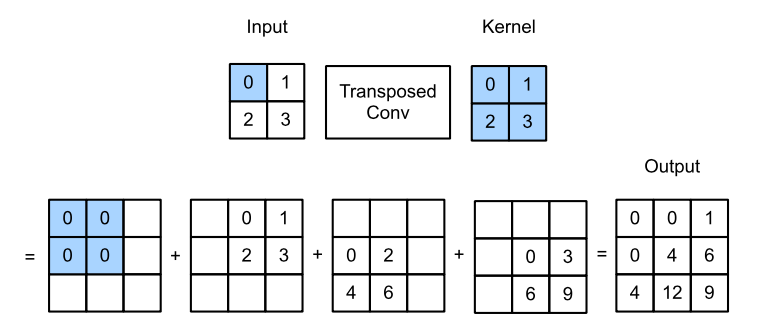
\includegraphics[width=0.8\textwidth]{transposed-conv}
  \caption{Transposed Convolution}
  \label{fig:trans-conv}
\end{figure}


\subsection{Fully Convolutional Networks}
\label{sec:fully-conv-netw}

A fully convolutional network (FCN) uses a convolutional neural network to transform image pixels to pixel classes.
Figure \ref{fig:fcn} shows the fully convolutional network.

\begin{figure}[!htbp]
  \centering
  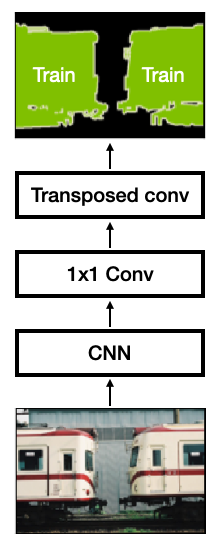
\includegraphics[width=0.3\textwidth]{fcn}
  \caption{FCN}
  \label{fig:fcn}
\end{figure}


%%% Local Variables:
%%% mode: latex
%%% TeX-master: "deep-learning"
%%% End:


\chapter{Generative Model}

\section{GAN}
\label{sec:gan}

\section{Diffusion Model}
\label{sec:diffusion-model}




\part{Natural Language Processing Practice}
\label{part:natur-lang-proc}

\chapter{Classificatrion}



\chapter{Chat}





% Pages are numbered with Arabic numbers.
% Chapters generate a table of contents entry but don't get a number.
\backmatter{}
\cleardoublepage{}
\phantomsection{}
\nocite{*}
\bibliographystyle{plain}       % % plain, unsrt, alpha, abbrv
\bibliography{tex}

\cleardoublepage{}
% just setting an anchor like \hypertarget{}{}
% fix the problem that anchor point to the previous section
\phantomsection{}                 
\printindex{}
\end{document}

%%% Local Variables:
%%% mode: latex
%%% TeX-master: t
%%% End:


